\documentclass{article}

% Language setting
% Replace `english' with e.g. `spanish' to change the document language
\usepackage[english]{babel}

% Set page size and margins
% Replace `letterpaper' with `a4paper' for UK/EU standard size
\usepackage[letterpaper,top=2cm,bottom=2cm,left=3cm,right=3cm,marginparwidth=1.75cm]{geometry}

% Useful packages
\usepackage{amsmath}
\usepackage{graphicx}
\usepackage[colorlinks=true, allcolors=blue]{hyperref}
\usepackage[normalem]{ulem}
\usepackage{listings}
\usepackage{color}
% \usepackage{flafter}

\definecolor{dkgreen}{rgb}{0,0.6,0}
\definecolor{gray}{rgb}{0.5,0.5,0.5}
\definecolor{mauve}{rgb}{0.58,0,0.82}

\lstset{frame=tb,
  language=Python,
  aboveskip=3mm,
  belowskip=3mm,
  showstringspaces=false,
  columns=flexible,
  basicstyle={\small\ttfamily},
  numbers=none,
  numberstyle=\tiny\color{gray},
  keywordstyle=\color{blue},
  commentstyle=\color{dkgreen},
  stringstyle=\color{mauve},
  breaklines=true,
  breakatwhitespace=true,
  tabsize=3
}

\title{Dijkstra in Disney World}
\author{Elizabeth Qiu}

\begin{document}
\maketitle

\begin{abstract}
For my final math project, I may or may not have started the project on the day of the due date. I'm procrastinating, yet always trying to find the most efficient and easiest way to get things done. So I thought it would be fitting to write about finding the shortest path for X. I am going to write about Dijkstra's algorithm.
\end{abstract}

\section{Introduction}

Say I wanted to go from my home (point A) to Disney World (point B). It would be a shame for Google Maps to first take me to Niagara Falls, and then to Seattle, before directing me to Orlando, Florida. In fact, I think Google would be bankrupt by now if it offered that quality of a service.

But let's say that there's a huge traffic jam all throughout US Route 301 (Maryland to Florida), and now I have to be stuck in the long line of cars. If I take a slightly longer method using local roads, I may actually end up at Disney World faster than using the inefficient highway.

That is where Dijkstra's algorithm comes in handy! It is all about getting from point A to B using the fastest method.

\section{The Basics}

\subsection{Credit where it's due}

Dijkstra's algorithm was developed by Edsger Dijkstra. He was a prominent Dutch computer scientist, software engineer, systems scientist, and science essayist \sout{and balloon artist}.

\subsection{Background}

Unlike breadth-first search that looks out for the shortest path with the fewest segments, Dijkstra's algorithm sets out to find the shortest path with the lowest cost in terms of weights. Dijkstra's algorithm only works on weighted graphs, while breadth-first search is handy for unweighted graphs. For the algorithm to work, the edges must also be directed, and must not have negative weight values.

\subsection{The algorithm}

Dijkstra's algorithm is consisted of 4 iterable steps for a graph. Also, the implementation is very complicated, as least for me. So, I've used pseudo-code instead of a real language. \dots

\begin{figure}
    \centering
    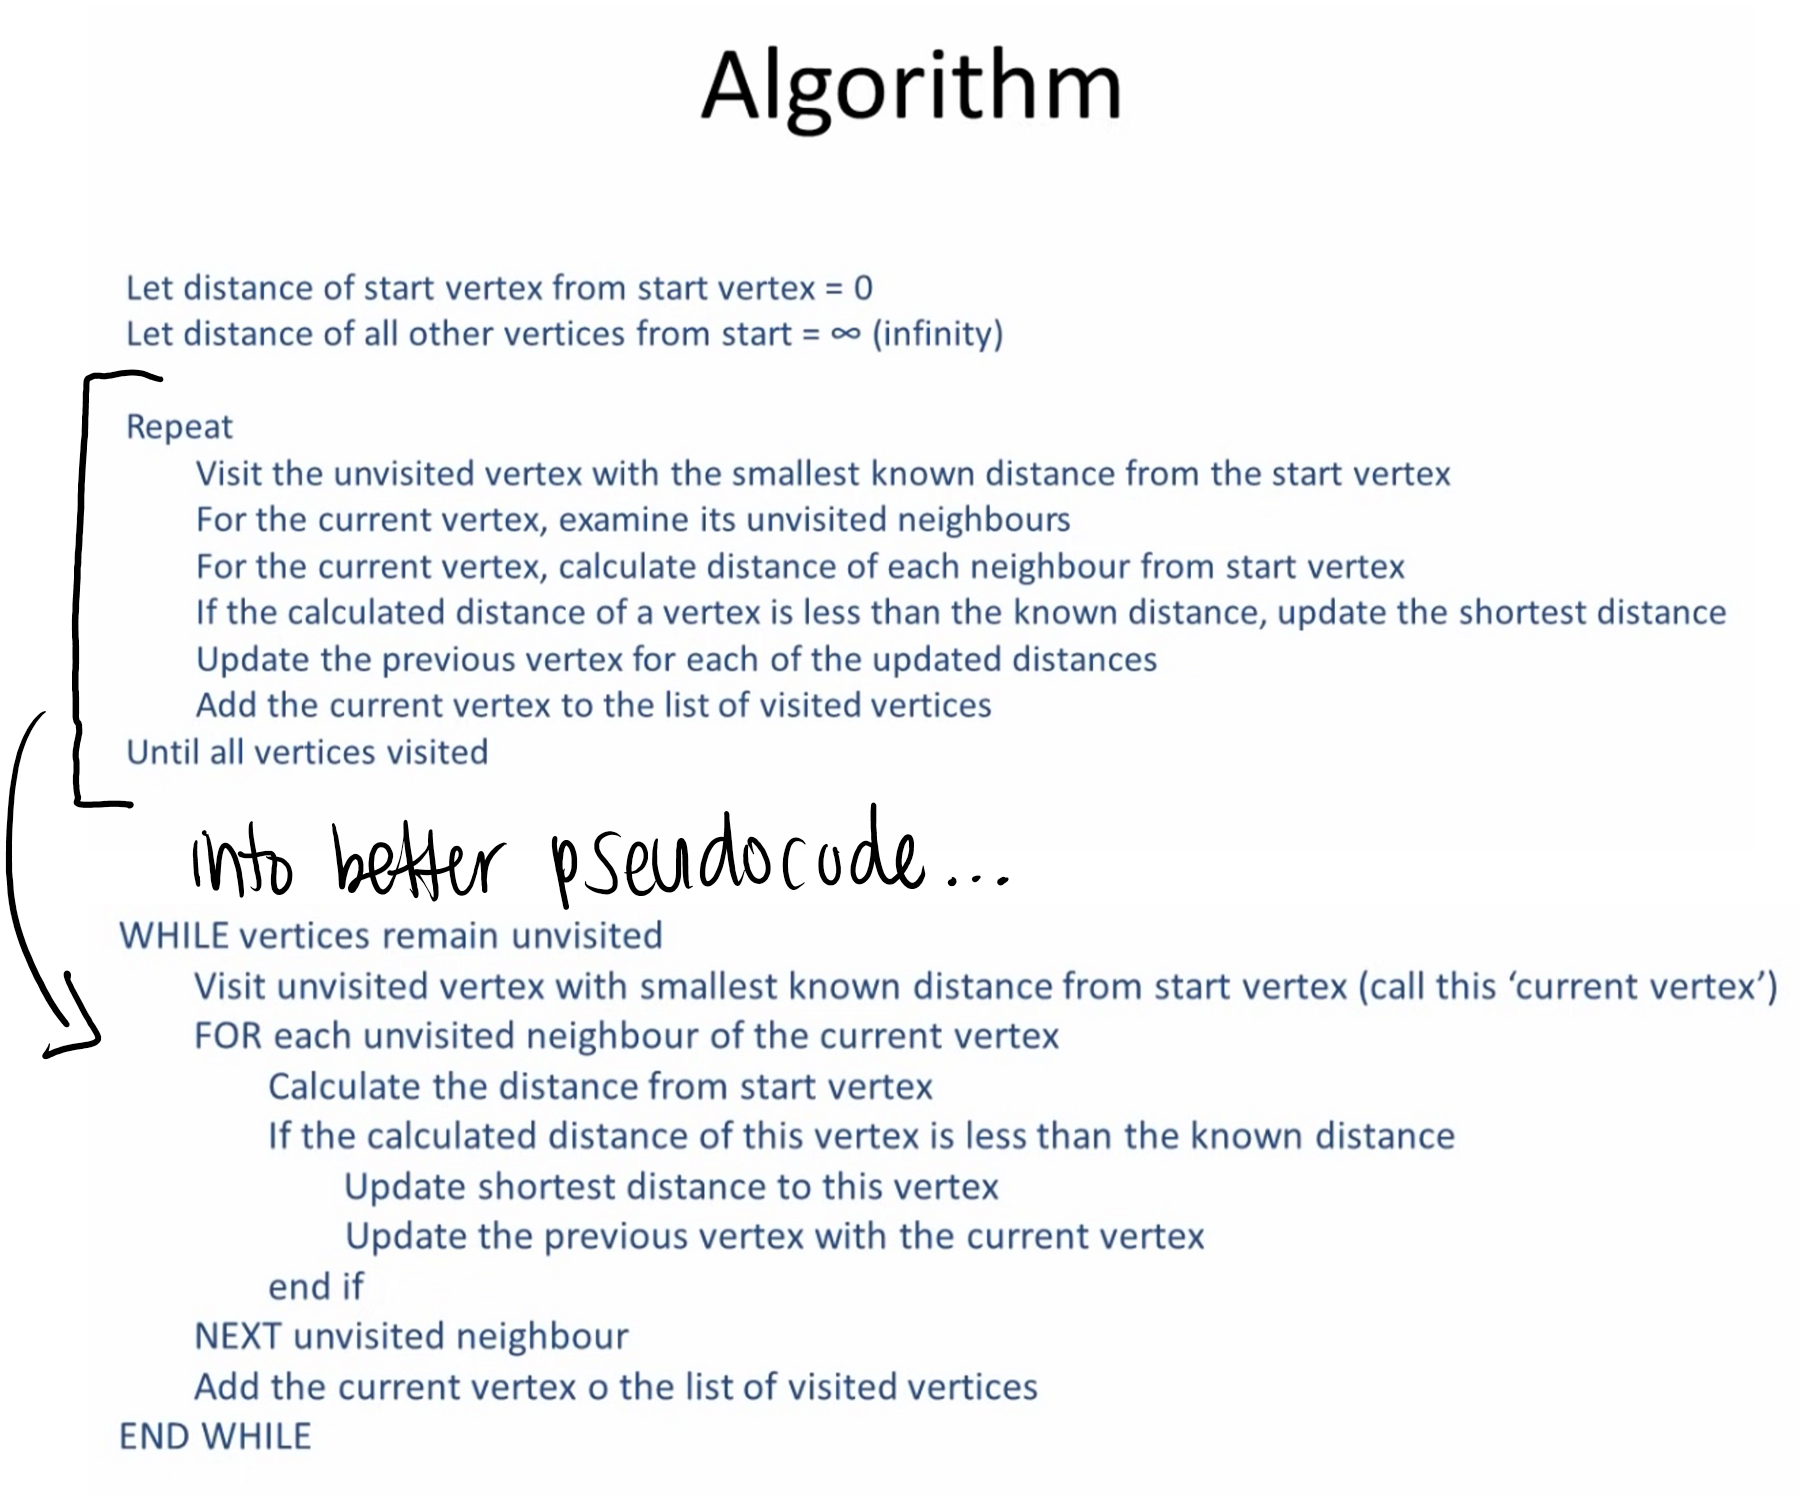
\includegraphics[width=0.6\textwidth]{algo.png}
    \caption{The algorithm described from words to pseudo-code. Credits: A YouTube video}
    \label{fig:my_label}
\end{figure}

\begin{enumerate}
    \item Find the "cheapest" node — the node that you can get to in the least amount of time.
    \item Check if there's a cheaper path to the neighbors of the node. If so, update the costs.
    \item Repeat steps 1-2 until you've gone through every node in the graph.
    \item Add together the weights to find the value of the final (cheapest) path.
\end{enumerate}

\subsection{Implementation}

If you watch the video, this will make much more sense! We'll be taking a trip from Maryland (or DC) to Disney World in Florida. For Dijkstra's algorithm, we need 3 hash tables,
\begin{enumerate}
    \item Graph
    \item Costs
    \item Parents
\end{enumerate}
where a hash table is a data structure that stores key-value pairs with a hash function.

\begin{figure}
    \centering
    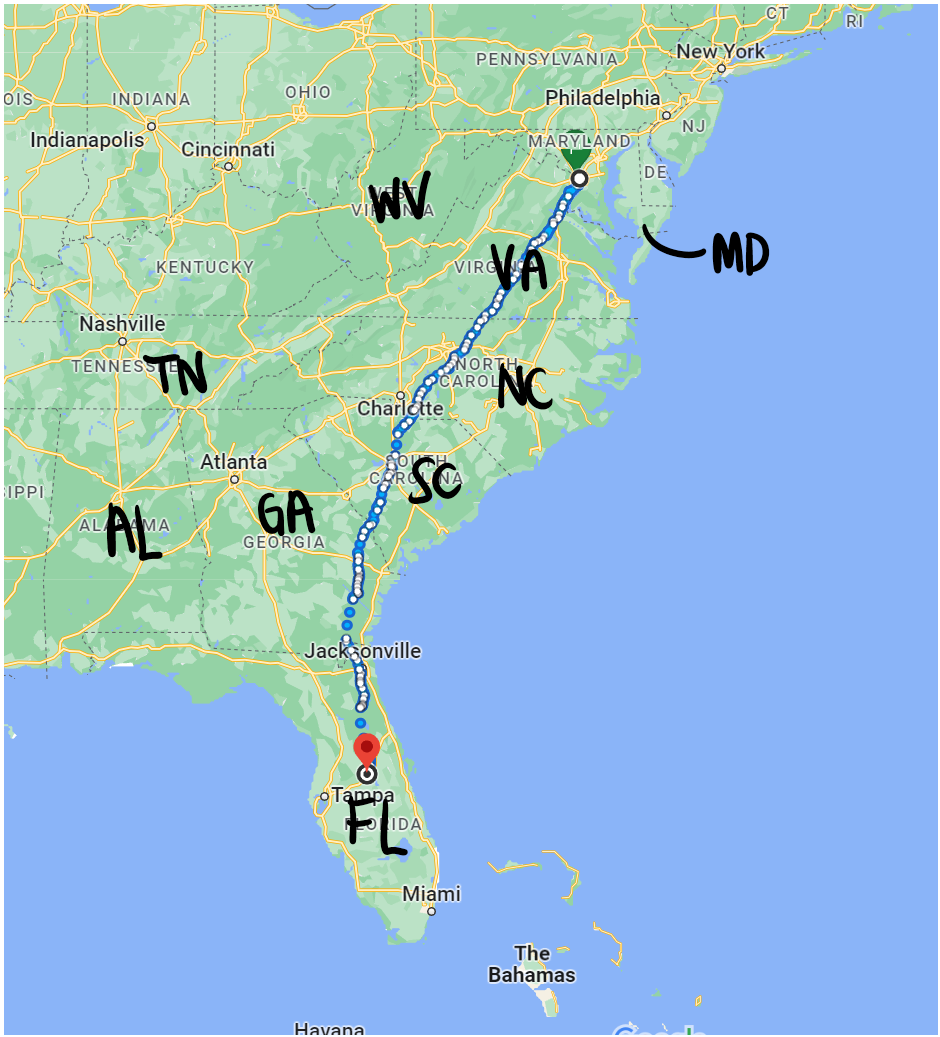
\includegraphics[width=0.5\textwidth]{map.png}
    \caption{\label{fig:map}This map was uploaded via the file-tree menu.}
\end{figure}

\begin{figure}
    \centering
    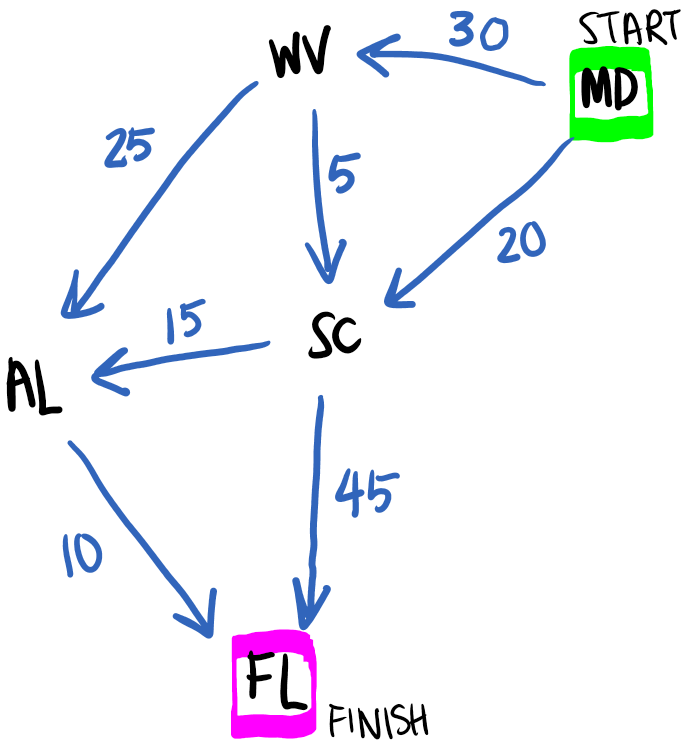
\includegraphics[width=0.5\textwidth]{nodes.png}
    \caption{\label{fig:nodes}For calculation purposes, VA, NC, TN, and GA do not exist (sorry!) — this is what a graph of the map above may look like.}
    \label{fig:my_label}
\end{figure}

\begin{figure}
    \centering
    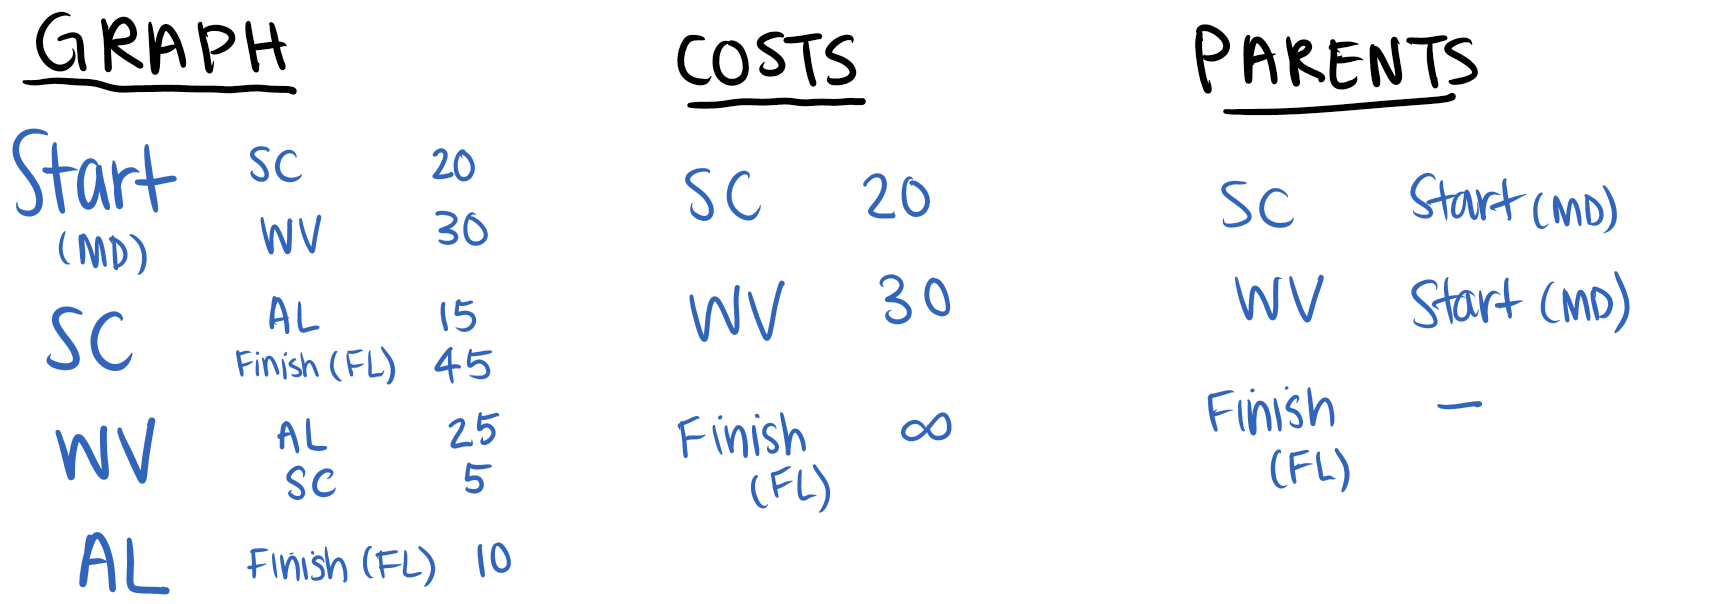
\includegraphics[width=0.7\textwidth]{3hashtables.png}
    \caption{From the information on the graph, these are the 3 hash tables we have generated.}
    \label{fig:my_label}
\end{figure}

% % cool easy way to implement code
% \begin{verbatim}
% your
% code
% example
% \end{verbatim}

% python code
\begin{lstlisting}
# dijkstra.python
# PLEASE NOTE: this will not actually run because i didn't completely define some stuff :)
# credits: Grokking Algorithms

# dictionary
parents = {}
parents["a"] = "start"
parents["b"] = "start"
parents["fin"] = None

# array
processed = []

node = find_lowest_cost_node(costs)
while node is not None:
    cost = costs[node]
    neighbors = graph[node]
    for n in neighbors.keys():
        new_cost = cost + neighbors[n]
        if costs[n] > new_cost:
            costs[n] = new_cost
            parents[n] = node
    processed.append(node)
    node = find_lowest_cost_node(costs)


def find_lowest_cost_node(costs):
    lowest_cost = float("inf")
    lowest_cost_node = None
    for node in costs:
        cost = costs[node]
        if cost < lowest_cost and node not in processed:
            lowest_cost = cost
            lowest_cost_node = node
    return lowest_cost_node

\end{lstlisting}

\subsection{Thank you!}

Thanks for reading! I hope you got a little better idea of how Dijkstra's algorithm works.

% \bibliographystyle{alpha}
% \bibliography{bibliography}

\begin{thebibliography}{widest entry}
 \bibitem[1]{1} "Grokking Algorithms" by Aditya Y. Bhargava
 \bibitem[2]{2} "Dijkstra’s Shortest Path Algorithm", a YouTube video made by the Computer Science channel
 ...
\end{thebibliography}


\end{document}